\section{Urnenmodelle}

Ein ``Urnenmodell'' ist eine abstrakte Darstellung von Zufallsexperimenten, bei denen zufällig Stichproben aus einer gegebenen Menge ``gezogen'' werden.
Eine Urne ist ein Behältnis in welchem sich farbige/nummerierte Kugeln befinden, die ansonsten ununterscheidbar sind.
Aus der Urne ziehe man blind/zufällig eine oder mehrere Kugeln und notiere ihre Farbe/Zahl.

\begin{center}
    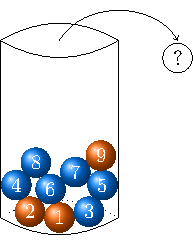
\includegraphics{./stoch_abbildungen/urne_mit_kugeln.pdf}
    \captionof{figure}{Urnenmodell mit nummerierten, farbigen Kugeln}
\end{center}

\subsection{Urnenmodell mit Zurücklegen: Multinomial-Verteilung}

Gegeben sei eine Urne mit $N$ Kugeln, verschiedenfarbig mit Farben aus $E$, wobei $\abs{E} \ge 2$ 

Man ziehe $n$ Stichproben/Kugeln, wobei nach jedem Zug die Kugel wieder zurückgelegt wird. Uns interessiert die Farbe in jedem Zug, setze also
\begin{equation*}
	\Omega = E^n \und \ereignisF = \pows\Omega 
\end{equation*}
Zur Bestimmung eines geeigneten Wahrscheinlichkeitsmaßes nummerieren wir die Kugeln mit $1,\dots, N$, so dass alle Kugeln der Farbe $a \in E$ eine Nummer aus $F_{a} \subset \menge{1,\dots, N}$ tragen. Würden wir die Nummern notieren, so wäre
\begin{equation*}
	\quer{\Omega} = \menge{1,\dots, N}^n \und \quer{\ereignisF} = \pows{\quer{\Omega}}
\end{equation*}
und wir könnten die Gleichverteilung $\quer{\P} = U(\quer{\Omega})$ als WMaß für einem einzelnen Zug verwenden. Für den Übergang zu $\Omega$ konstruieren wir  Zufallsvariablen. Die Farbe im $i$-ten Zug wird beschrieben durch
\begin{equation*}
	\bigabb{X_i}{\quer{\Omega}}{E}{\quer{\omega} = \left( \quer{\omega}_1, \dots, \quer{\omega}_n \right)}{a \enskip \text{ falls } \quer{\omega}_i \in F_a}
\end{equation*}
Der Zufallsvektor
\begin{equation*}
	\abb{X = (X_1, \dots, X_n)}{\quer{\Omega}}{\Omega}
\end{equation*}
beschreibt dann die Abfolge der Farben. Für jedes $\omega \in \Omega$ gilt dann
\begin{equation*}
	\menge{X = \omega} = F_{\omega_1} \times \cdots \times F_{\omega_n} = \bigtimes_{i=1}^{n} F_{\omega_i}
\end{equation*}
und damit
\begin{equation*}
    \P(\menge{\omega}) 
    = \quer{\P}(X^{-1}(\menge{\omega})) = \P(X=\omega)
    = \frac{\abs{F_{\omega_1}} \cdots \abs{F_{\omega_n}}}{\abs{\quer{\Omega}}}
    = \prod_{i=1}^{n} \frac{\abs{F_{\omega_i}}}{N} 
    \defqe \prod_{i=1}^{n} \rho(\omega_i)
\end{equation*}
Zähldichten, die sich als Produkt von Zähldichten schreiben lassen, werden auch als \begriff{Produktdichten} bezeichnet ($\nearrow$  \S 3 Unabhängigkeit).

Sehr oft interessiert uns bei einem Urnenexperiment nicht die Reihenfolge der gezogenen Farben, sondern nur die Anzahl der Kugeln in Farbe $a \in E$ nach $n$ Zügen. Dies entspricht
\begin{equation*}
	 \dach{\Omega} 
	 = \menge{k = (k_a)_{a \in E} \in \N_{0}^{\abs{E}} \colon \sum_{a \in E} k_a = n}
	 \und \dach{\ereignisF} = \pows{\dach{\Omega}}
\end{equation*}
Den Übergang $\Omega \to \dach{\Omega}$ beschreiben wir durch die Zufallsvariablen
\begin{equation*}
	\bigabb{Y_a(\omega)}{\Omega}{\N_{0}}%
    {\omega = (\omega_1,\dots, \omega_n)}%
    {\sum_{a \in E} \one_{\menge{a}}(\omega_i)} 
\end{equation*}
und
\begin{equation*}
	\abb{Y = (Y_a)_{a \in E}}{\Omega}{\dach{\Omega}}
\end{equation*}
Wir erhalten
\begin{equation*}
	\begin{aligned}
		\P(Y=k) &= \P(Y_a = k_a : a \in E) \\
		&= \sum_{\omega \in \Omega \colon Y(\omega) = k} \prod_{i=1}^ \rho(\omega_i)
		= \sum_{\omega \in \Omega \colon Y(\omega) = k} \prod_{a \in E} \rho(a)^{k_a} 
		= \binom{n}{\folge{k_a}[a \in E]} \prod_{a \in E} \rho(a)^{k_a}
	\end{aligned}
\end{equation*}
wobei
\begin{equation*}
	\binom{n}{(k_1 , \dots , k_l)} \defeq \begin{cases}
	\frac{n!}{k_1 ! \cdots k_l !} & \text{falls } \sum_{i=1}^l k_i = 1 \\
	0 & \text{sonst}
	\end{cases}
\end{equation*}
der Multinomialkoeffizient ist, welcher die Anzahl der Möglichkeiten beschreibt $n$ Objekte in $l$ Gruppen aufzuteilen, sodass die Gruppe $i$ gerade $k_i$ Objekte enthält.

\begin{definition}
	Sei $l \geq 2$, $p=(p_1 , \dots , p_l)$ eine Zähldichte und $n \in \N$, dann heißt die Verteilung auf 
	\begin{equation*}
		\menge{k=\folge{k_i}[i=1, \dots , l] \in \N_0^l : \sum_{i=1}^l k_i = 1}
	\end{equation*}
	mit Zähldichte
	\begin{equation*}
		m((k_1 , \dots , k_l)) = \binom{n}{k_1 , \dots , k_l} \prod_{i=1}^l p_i^{k_i}
	\end{equation*}
	\begriff{Mulitnomialverteilung} mit Parametern $n$ und $p$. Wir schreiben auch $\Multi(n,p)$.
\end{definition}

\begin{beispiel}
	Eine Urne enthalte nur schwarze (``1'') und weiße (``0'') Kugeln ($E = \menge{0,1}$) und es sei $\rho(1) = p$ gerade die Proportion der schwarzen Kugeln (Wahrscheinlichkeit bei einem Zug schwarz zu ziehen). Dann ist die Wahrscheinlichkeit in $n$ Zügen $k$-mal schwarz zu ziehen
	\begin{equation*}
		\binom{n}{k} \prod_{i=0,1} \rho(i)^{k_i} = \binom{n}{k} *p^k * (1-p)^{n-k}
	\end{equation*}
	Ein solches (wiederholtes) Experiment mit nur zwei möglichen Ergebnissen und feste Wahrscheinlichkeit $p \in [0,1]$ nennen wir auch (wiederholtes) \person{Bernoulli}-Experiment.
\end{beispiel}

\begin{definition}
	Sei $p \in [0,1]$ und $n \in \N$, dann heißt die Verteilung mit Zähldichte
	\begin{equation*}
		\rho(k) = \binom{n}{k} p^k (1-p)^{n-k} \qquad k \in \menge{0, 1 , \dots , n}
	\end{equation*}
	\begriff{Binomialverteilung} auf $\menge{0, \dots, n}$ mit Parameter $p$ (Erfolgswahrscheinlichkeit). Wir schreiben auch $\Bin(n,p)$. Im Fall $n=1$ nennen wir die Verteilung mit Zähldichte
	\begin{equation*}
		\rho(0) = 1-p \quad \rho(1) = p
	\end{equation*}
	auch \begriff{Bernoulliverteilung} mit Parameter $p$ und schreiben $\Bernoulli(p)$.
\end{definition}

\subsection{Urnenmodell ohne Zurücklegen: Hypergeometrische Verteilung}
Gegeben sei ein Urne mit $N$ Kugeln verschiedener Farben aus $E$ mit $\card{E} \geq 2$. Es werden $n \leq N$ Stichproben entnommen, wobei die gezogenen Kugeln nicht in die Urne zurückgelegt werden.

\begin{beispiel}
	Eine Urne enthalte $S$ schwarze (``1'') und $W$ weiße (``0'') Kugeln, d.h. $E = \menge{0,1}$ und $S+W=N$. Dann ist die Wahrscheinlichkeit in $n$ Zügen ohne Zurücklegen gerade $s$ schwarze und $w$ weiße Kugeln zu ziehen
	\begin{equation*}
		\rho(s) = \frac{\binom{W}{w} * \binom{S}{s}}{\binom{N}{n}} \qquad 0 \leq s \leq S, 0 \leq w \leq W, s+w=n, S+W=N
	\end{equation*}
\end{beispiel}

\begin{definition}
	Seien $N \in \N, W \leq N, n \leq N$. Dann heißt die Verteilung auf $\menge{0, \dots , n}$ mit Zähldichte 
	\begin{equation*}
		\rho(w) = \frac{\binom{W}{w} * \binom{N-W}{n-w}}{\binom{N}{n}} \qquad w = \max\menge{0 , n-N+W} , \dots \min\menge{W,n}
	\end{equation*}
	\begriff{Hypergeometrische Verteilung} mit Parametern $N,W$ und $n$. Wir schreiben auch $\Hyper(N,W,n)$.
\end{definition}